% \documentclass[lineno,twocolumn,endfloat,biblatex]{biophys-new}
\documentclass{biophys-new}
\usepackage[utf8]{inputenc}
\usepackage{graphicx}
\usepackage[colorlinks,allcolors=cyan!70!black]{hyperref}

% Uncomment if using biblatex
% \addbibresource{sample.bib}

\usepackage{lipsum}

\title{Correlation in the subunit dynamics of SARS-CoV-2 main protease}
\runningtitle{Biophysical Journal Template} %% For page header

\author[1,]{Jason G. Pattis}
\author[1,*]{Vincent A. Voelz}
\runningauthor{Author1 and Author2} %% For page header

\affil[1]{Temple University, Philadelphia, Pennsylvania 19122, USA}


\corrauthor[*]{voelz@temple.edu}

% \papertype{Letters}
\papertype{Article}
% \papertype{Computational Tools}


\begin{document}

\begin{frontmatter}

\begin{abstract}
Each 
\end{abstract}

\begin{sigstatement}
no more than 120 words.
\end{sigstatement}
\end{frontmatter}

\section*{Outline}

\begin{enumerate}
    \item What are the rare event motions which occur in the main protease dimer?
    \begin{itemize}
        \item the slowest motion is the folding of the linker helix (residue 188 to 194) this motion is IC 1 and IC 2
        \item This helix is also found in the infectious bronchitis virus (IBV) crystal structure when IBV is in its monomeric state
        \item the second slowest motion (IC 3) is a change in residue 140
        \item These motions are not symmetric (they only occur in one monomer) 
        \item Are these motions connected to active site dynamics and active site opening?
        \begin{itemize}
            \item Mutual information would suggest that many residues far from the active site have correlated motions with the active site
            \color{blue}
            \item look at active site pocket volume
            \item look at 145 to 41 distance as proxy for open to substrate
            \item look at 3 10 helix formation (139-141) as proxy for active
        \end{itemize}
    
    \end{itemize}
    \item How often do these motions occur?
    \begin{itemize}
        \item The slowest motions occur only once in the 100 us trajectory
    \end{itemize}
    \item Can people dock to the different conformations seen in this simulation?
    \begin{itemize}
        \item Yes cluster centers and populations well be available online for ensemble docking
        \begin{itemize}
            \color{blue}
            \item cluster centers will have to be pushed to osf or similar because they are to big for github
        \end{itemize}
    \end{itemize}
    \item Are there correlated motions creating an allosteric network? Can these allosteric regions affect the active site and the activity of the enzyme
    \begin{itemize}
        \item Mutual information analysis reveals correlated motions within the active site and residues 232 to 238
        \begin{itemize}
            \color{blue}
            \item Is there a pocket near 232 to 238
        \end{itemize}
    \end{itemize}
    \item Is there evidence that only one monomer is active at a time?
     \begin{itemize}
        \item look for alternating:
        \begin{itemize}
            \color{blue}
            \item active pocket volume
            \item res 41 to 145 distance
            \item 3 10 helix formation (139-141)
            \item packing between His163 and Phe140 may transfer conformational change to other monomer
        \end{itemize}
    \end{itemize}
\end{enumerate}


\section*{Introduction}

Covid-19 has been a massive public health threat all around the globe. Covid-19 is caused by the Sars-Cov-2 virus, a member of the $\MakeUppercase{\beta}$-Coronavirus family of viruses. Therapeutics are desperately needed. One promising target for drug development is Sars-Cov-2's non-structuralprotein 5 (Nsp5), also called the main protease or $M_{pro}$, or the 3CL-like protease ($3CL_{pro}$) because of its similarity to 3C proteases of picornaviruses\cite{tan2005ph}. The Sars-Cov-2 genomic RNA is transcribed into large polyproteins, which contains many different proteins. The $M_{pro}$ is responsible for cutting the polyproteins, an essential step the the virus' life cycle to make these proteins functional. Humans do not have a similar protease, which makes $M_{pro}$ an attractive drug target. One $M_{pro}$ inhibitor has entered phase I clinical trials \cite{boras2020discovery} and large collaborative efforts to find other inhibitors are underway\cite{achdout2020covid}.

Sars-Cov-2 is an enveloped virus with a positive-sense RNA genome protected by a neculeoprotein. Sars-Cov-2's RNA dependent RNA polymerase transcribes two overlapping polyproteins (pp1a and pp1ab) which need to be cleaved before they are functional. the Main protease cuts at the sequence Leu-Gln/Ser-Ala-Gly  where / is the cleavage point\cite{Zhang409}. The Leucine at position 2 has very high specificity but the preceding residues do play a role in binding but can be many different amino acids \cite{rut2020substrate}. The $M_{pro}$ makes cuts at 11 different sites across pp1a and pp1ab. In addition, no host-cell proteases are known to have the same recognition sequence making this a great drug target\cite{hilgenfeld2014sars}. 

The first crystal structure of the Sars-cov-2 $M_{pro}$ became available in March, 2020 \cite{Zhang409} with more structures quickly following\cite{owen2020sars}\cite{jin2020structure}, it showed an extremely similar structure to the Sars-Cov $M_{pro}$ (PDB entry 2BX4)\cite{tan2005ph} at 0.53 Å RMSD for all C$\alpha$ and has a 96\% sequence identity\cite{Zhang409}. $M_{pro}$ has 3 domains. Domain I (residues 10 to 99) and domain II (residues 100 to 182) are both anti-parallel $\MakeUppercase{\beta}$-barrels with the active site in between them. The peptide Substrate binding site is labeled with different pockets where the residues bind; S4, S3, S2, and S1 (for Substrate binding site 1, etc.) leading up to the cleavage site and S1', S2' after. The corresponding substrate or inhibitor moiety that binds to S1 is labeled P1 for protein binding site 1. The catalytic residues are His41 on domain I and Cys145 on domain II. The steps of the catalysis by Cys145 and His41 have been studied and detailed through quantum mechanics calculations. \cite{swiderek2020revealing} Domain II is the primary domain responsible for dimerization. Domain II and III have a long linker loop in between them. Domain III (residues 198 to 303) also creates contacts to help stabilize the dimer and has been implicated in regulating dimerization as well as being able to allostericly regulate catalysis.

Mutagaenesis on another caronavirus, gastroenteritis virus, $M_{pro}$ suggests Domain III helps maintain the shape of loop 184-199 (the long linker between domain II and III), with help from the N-terminal residues. Asp186 makes a salt bridge to Arg40 that appears to be required to maintain the active site geometry and is involved in substrate binding. \cite{anand2002structure}.

In Sars-Cov the contacts between the two domain IIIs (Ser284,Thr285,Ile286) when mutated to alanine, bring the two domains III's closer together and increase activity.\cite{shi2006catalysis} It is believed that the increase in activity is due to an increase in concentration of dimer vs monomer, which was supported by analytical ultracentrifugation \cite{hsu2005critical}. Many residues directly adjacent to this region can also affect activity. Phe291A contacts the N-terminus and increases activity. Glu288A, Asp289A, Glu290A, Arg298A, Gln299A all cause a large reduction in activity. Deletion of the N or C termini reduces dimerization and also catalytic activity.\cite{shi2006catalysis}\cite{shi2004dissection} This may suggest a connection from domain III to the N terminus to the active site as Arg4 contacts Glu290, Asn214 contacts Phe3 and Gln299, while Glu288 contacts Lys5. Residue 285 in Sars-Cov-2 is an Alanine bringing domain III closer than Sars-Cov, however the catalytic efficiency of Sars-Cov-2 is only marginally higher than Sars-Cov \cite{Zhang409} 

The monomeric $M_{pro}$ is not active, only the dimer is active.\cite{chen2006only} In addition, dimerization is very strong with a $K_{d}$ of 2.5 µM measured by analytical ultracentrifugation \cite{Zhang409} Their is some evidence that the monomer and dimer take on different conformations. The coronavirus, infectious bronchitis virus was crystallized with three monomers in the asymmetric unit, a dimer (chain A and B) and a monomer (chain C)\cite{xue2008structures}. The monomer contains a short helix (residues 186 to 190) in the linker loop between domain II and III. In addition, domain III shifted 5 Å away from domains I and II, without much internal conformational change. IBV causes avian coronavirus and is part of the $\MakeUppercase{\gamma}$coronaviurs family.

Furthermore, in Sars-Cov there has also been some evidence from enzyme assays that in the dimer only one monomer is active at a time\cite{chen2006only}. A crystal structure of Sars-Cov has also shown some asymmetries, most notably a $3_{10}$ helix forming in residues 139-141, and is believed to be a sign of inactivation. \cite{yang2003crystal}. Having only one monomer active at a time has been seen in other dimeric enzymes and is believed to balance the entropic penalty of being ordered during catalysis by increasing the disorder in the other monomer.\cite{kim2017role}

Several studies have learned about the dynamics of $M_{pro}$ using molecular dynamics simulations. A simulation using the enhanced sampling technique Gaussian accelerated molecular dynamics was able to identify three pockets, the active site, a pocket at the dimer interface, and a pocket in the center of domain III. The authors observed correlated motions between domain I and domain III in monomer simulations but not the dimer simulations. Furthermore, these correlations do not change when $M_{pro}$ is bound to the inhibitor N3\cite{sztain2020elucidation}. Another study looked for sings of inactivation and found asymmetric differences primarily near the oxyanion hole. These include the distance from residue 166 to 172, 166 to 163, 145 to 41, and the pi stacking of residues 163 and 140.\cite{inizan2021high} It was found that the protonation of His172  impacts the conformation of the S1 pocket through an interaction network involving His172, Glu166, His163, and Phe140.\cite{verma2020proton} Novel states have been identified \cite{carli2020candidate, cocina2020sapphire} and the affects of mutations have also been examined. \cite{dubanevics2021computational, zhou2019identification}

Neutron scattering experiments would suggest that not all of the protonation states chosen for the D.E. Shaw simulation were the most likely protonation state.\cite{kneller2020unusual} That experiment suggests that His41 is protonated on both delta and epsilon nitrogens where as in the D.E. Shaw simulation it was modeled with the delta nitrogen deprotonated and epsilon nitrogen protonated. The other histadines (163, 164, and 172) were also modeled as delta nitrogen deprotonated. The neutron experiment suggest His163 would have its delta nigtogen protonated but not the epsilon nigtogen, His 164 would have both nitrogens protonated, and His172 was modeled correctly. All cystines were modeled as protonated but the neutron experiments suggest that Cys22, Cys38, Cys41, Cys44, and Cys128 should be deprotonated. Additional neutron experiments suggest that binding of an inhibitor can have a cascade of protonation/deprotonation.\cite{kneller2021direct}

Understanding the dynamics of this protein would be a massive benefit to drug discovery efforts. Dynamics of the active sight can inform how current compounds can be extended to make greater contact with the protein and improve affinity. Dynamics of the full protein provide insights into additional druggable pockets and how they are allostericly coupled to the active site. Furthermore additional insight into possible single monomer activation could help inform the design of experiments being run to test drug candidates.

\section*{Methods}

A 100 $\mu$S molecular dynamics simulation of the dimer $M_{pro}$ was run by D.E Shaw Research on the Anton 2 supercomputer.\cite{shaw2020molecular} The simulation used the DES-Amber all atom forcefield\cite{piana2020development} with explicit water and 0.15 M NaCl. The simulation was started from an apo crystal structure, pdbid: 6Y84. The simulation was run at 300 K in the NPT ensemble and frames were saved every 1 ns.

\subsection*{Discovery of slow motions}

Rare event conformational changes were found using the time-lagged independent component analysis (tica).\cite{perez2013identification,schwantes2013improvements} In order to find good internal coordinates to describe the system, or features, a few were tried and compared using the vamp-2 score.\cite{wu2020variational, scherer2019variational} Because a large number of features requires a extremely large amount of computer memory, Alpha carbon distances were filtered to select the most relevant. Distances of residue pairs which never come close to each other were filtered out, as well as distances which never change. The filtered distances (fdis) featurization includes only alpha carbon distances which had a minimum below 10 Å and a standard deviation above 0.35 Å, totaling 2389 distances. The more filtered distances (mfdis) includes only alpha carbon distances which had a minimum below 12 Å and a standard deviation above 0.30 Å, totaling 4618 distances. Feature selection was performed using the vamp-2 score\cite{wu2020variational, scherer2019variational} of the top 10 singular values of the vamp dimensionality reduction using 20 iterations of 50:50 shuffle split to avoid overfitting. This was repeated with lag times of 2, 8, and 16 ns. Multiple lag times were tested to ensure that trends were not lag time dependent, which they were not. Scores at different lag times can not be compared.\cite{husic2017note} Tica was performed on the fdis featurization with a lag time of 10 ns and using the commute map algorithm to scale the eigenvectors.\cite{noe2016commute} Tica solves the eigenvalue problem using a covariance matrix and a time-lagged covariance matrix to find rare event motions. To help interpret tica components correlations between input features, $X_i$ and the independent components, $\theta_j$, were calculated using the instantaneous, linear correlation between them written as:

\begin{equation}
\mathbf{Corr}(X_i - \mu_i, \mathbf{\theta}_j) = \frac{1}{\sigma_{X_i - \mu_i}}\sum_l \sigma_{(X_i - \mu_i)(X_l - \mu_l)} \mathbf{U}_{li}    
\end{equation}

The matrix U are the eigenvectors from tica. These calculations were done using PyEMMA version 2.5.7. \cite{scherer2015pyemma}

\subsection*{Discovery of correlated motions}

Correlated motions were found by calculating the mutual information between the backbone dihedrals of residue pairs with the MDEntropy package version 0.4.0.\cite{mdentropy} The mutual information is defined as the difference between the Shannon entropies (S) of the marginal distributions of variables (dihedrals of residues) X and Y and the joint Shannon entropy (equation 1)
\begin{equation}
I(X, Y)=S(X)+S(Y)-S(X, Y)
\end{equation}
I(X,Y) is calculated from the marginal and joint probabilities of the backbone dihidrals clustered into three bins (equation 2)
\begin{equation}
I(X, Y)=\sum_{x \in X} \sum_{y \in Y} p(x, y) \log \frac{p(x, y)}{p(x) p(y)}
\end{equation}
Frames were strided by 5 making frames 5 ns apart. the K-nearest neighbors algorithm was used to calculate entropy. statistically significance was ensured by subtracting the average mutual information values computed from five trials with scrambled data. In figure 5 MI < 0.05 was set to 0 for visual clarity

Exposons are pockets on a protein which only rarely open to become solvent exposed.\cite{porter2019cooperative, cruz2020discovery} Exposons were discovered by first calculating the mutual information between solvent exposed surface area per residue. Next, Affinity propagation was used to cluster the mutual information matrix into groups (exposons). The exposons were ranked from largest to smallest by how many residues were involved in each exposon. Exposons were calculated using Enspara 0.1.0.\cite{porter2019enspara}

\subsection*{Activation of a single monomer}

Distances were measured using MDtraj version 1.9.3.\cite{McGibbon2015MDTraj} Plots were made using matplotlib.\cite{Hunter:2007} Images were taken using VMD version 1.9.4\cite{HUMP96} and UCSF Chimera version 1.14.\cite{pettersen2004ucsf} Code for all analysis is available at: https://github.com/jgpattis/Desres-sars-cov-2-apo-mpro.

\section*{Results}

\begin{figure}[hbt!]
\centering
% figure made with: https://github.com/jgpattis/Desres-sars-cov-2-apo-mpro/blob/master/tica_plot_06.py
% raw image: raw_figures/fig_1_fdiscolortime_ic2.pdf
% raw_figures/fig_1_fdiscolortime_ic2.graffle
\includegraphics[width=0.6\linewidth]{figures/fig_1_fdiscolortime_ic2_label.png}
\caption{Motions of A) monomer A and B) monomer B in Independent component 1 and 2 space colored by simulation time. Numbered points represent cluster centers}
\label{fig:view}
\end{figure}

\begin{figure}[hbt!]
% alignment-along-ic1
% raw images: raw_figures/IC1_align_red46_orange12_yellow41.png
% raw_figures/Red46_blueStarting.png
% raw_figures/fig2_IC1_align.graffle
% pdb files: https://github.com/jgpattis/Desres-sars-cov-2-apo-mpro/tree/master/structure_08
\centering
\includegraphics[width=0.6\linewidth]{figures/fig2_IC1_align.png}
\caption{Alignment of chain B A) of cluster 46 (Red), 12 (orange), and 41 (yellow) and B) of cluster 46 (red) and the starting structure (blue)}
\label{fig:view}
\end{figure}

\begin{figure}[hbt!]
\centering
\includegraphics[width=0.6\linewidth]{images/blue-2Q6D-C-brown-cluster-41-better-align-2.png}
\caption{Alignment of infectious bronchitis virus, pdbid:2q6d.C (light blue) and chain B of cluster 41 (brown)}
\label{fig:view}
\end{figure}

\begin{figure}[hbt!]
% figure made with: https://github.com/jgpattis/Desres-sars-cov-2-apo-mpro/blob/master/tica_plot_06.py
% raw image: raw_figures/fig_4_fdiscolortime_ic3.pdb
% raw_figures/fig_4_fdiscolortime_ic3.gaffle
\centering
\includegraphics[width=0.6\linewidth]{figures/fig_4_fdiscolortime_ic3_label.png}
\caption{Motions of A) monomer A and B) monomer B in Independent component 1 and 3 space colored by simulation time. Numbered points represent cluster centers}
\label{fig:view}
\end{figure}

\begin{figure}[hbt!]
% mutual-information-heatmap
% script which creates image: https://github.com/jgpattis/Desres-sars-cov-2-apo-mpro/blob/master/allostery_analysis/plot_mut_info.py
% and : https://github.com/jgpattis/Desres-sars-cov-2-apo-mpro/blob/master/allostery_analysis/plot_mut_info_bothchain.py
% raw images : raw_figures/dmi_matrix.pdf
% raw_figures/dmi_bothchain_matrix.pdf
% raw_figures/MI_full_and_average.graffle
\centering
\includegraphics[width=0.6\linewidth]{figures/MI_full_and_average.png}
\caption{Correlated motions of residue residue pairs of A) chain A and B averaged together and B) the full dimer }
\label{fig:view}
\end{figure}

\begin{figure}[hbt!]
% exposons
% script which creates image: 
% https://github.com/jgpattis/Desres-sars-cov-2-apo-mpro/blob/master/cryptic_pockets/plot_exposons.py
% raw images : 
% raw_figures/dmi_bothchain_matrix.pdf
\centering
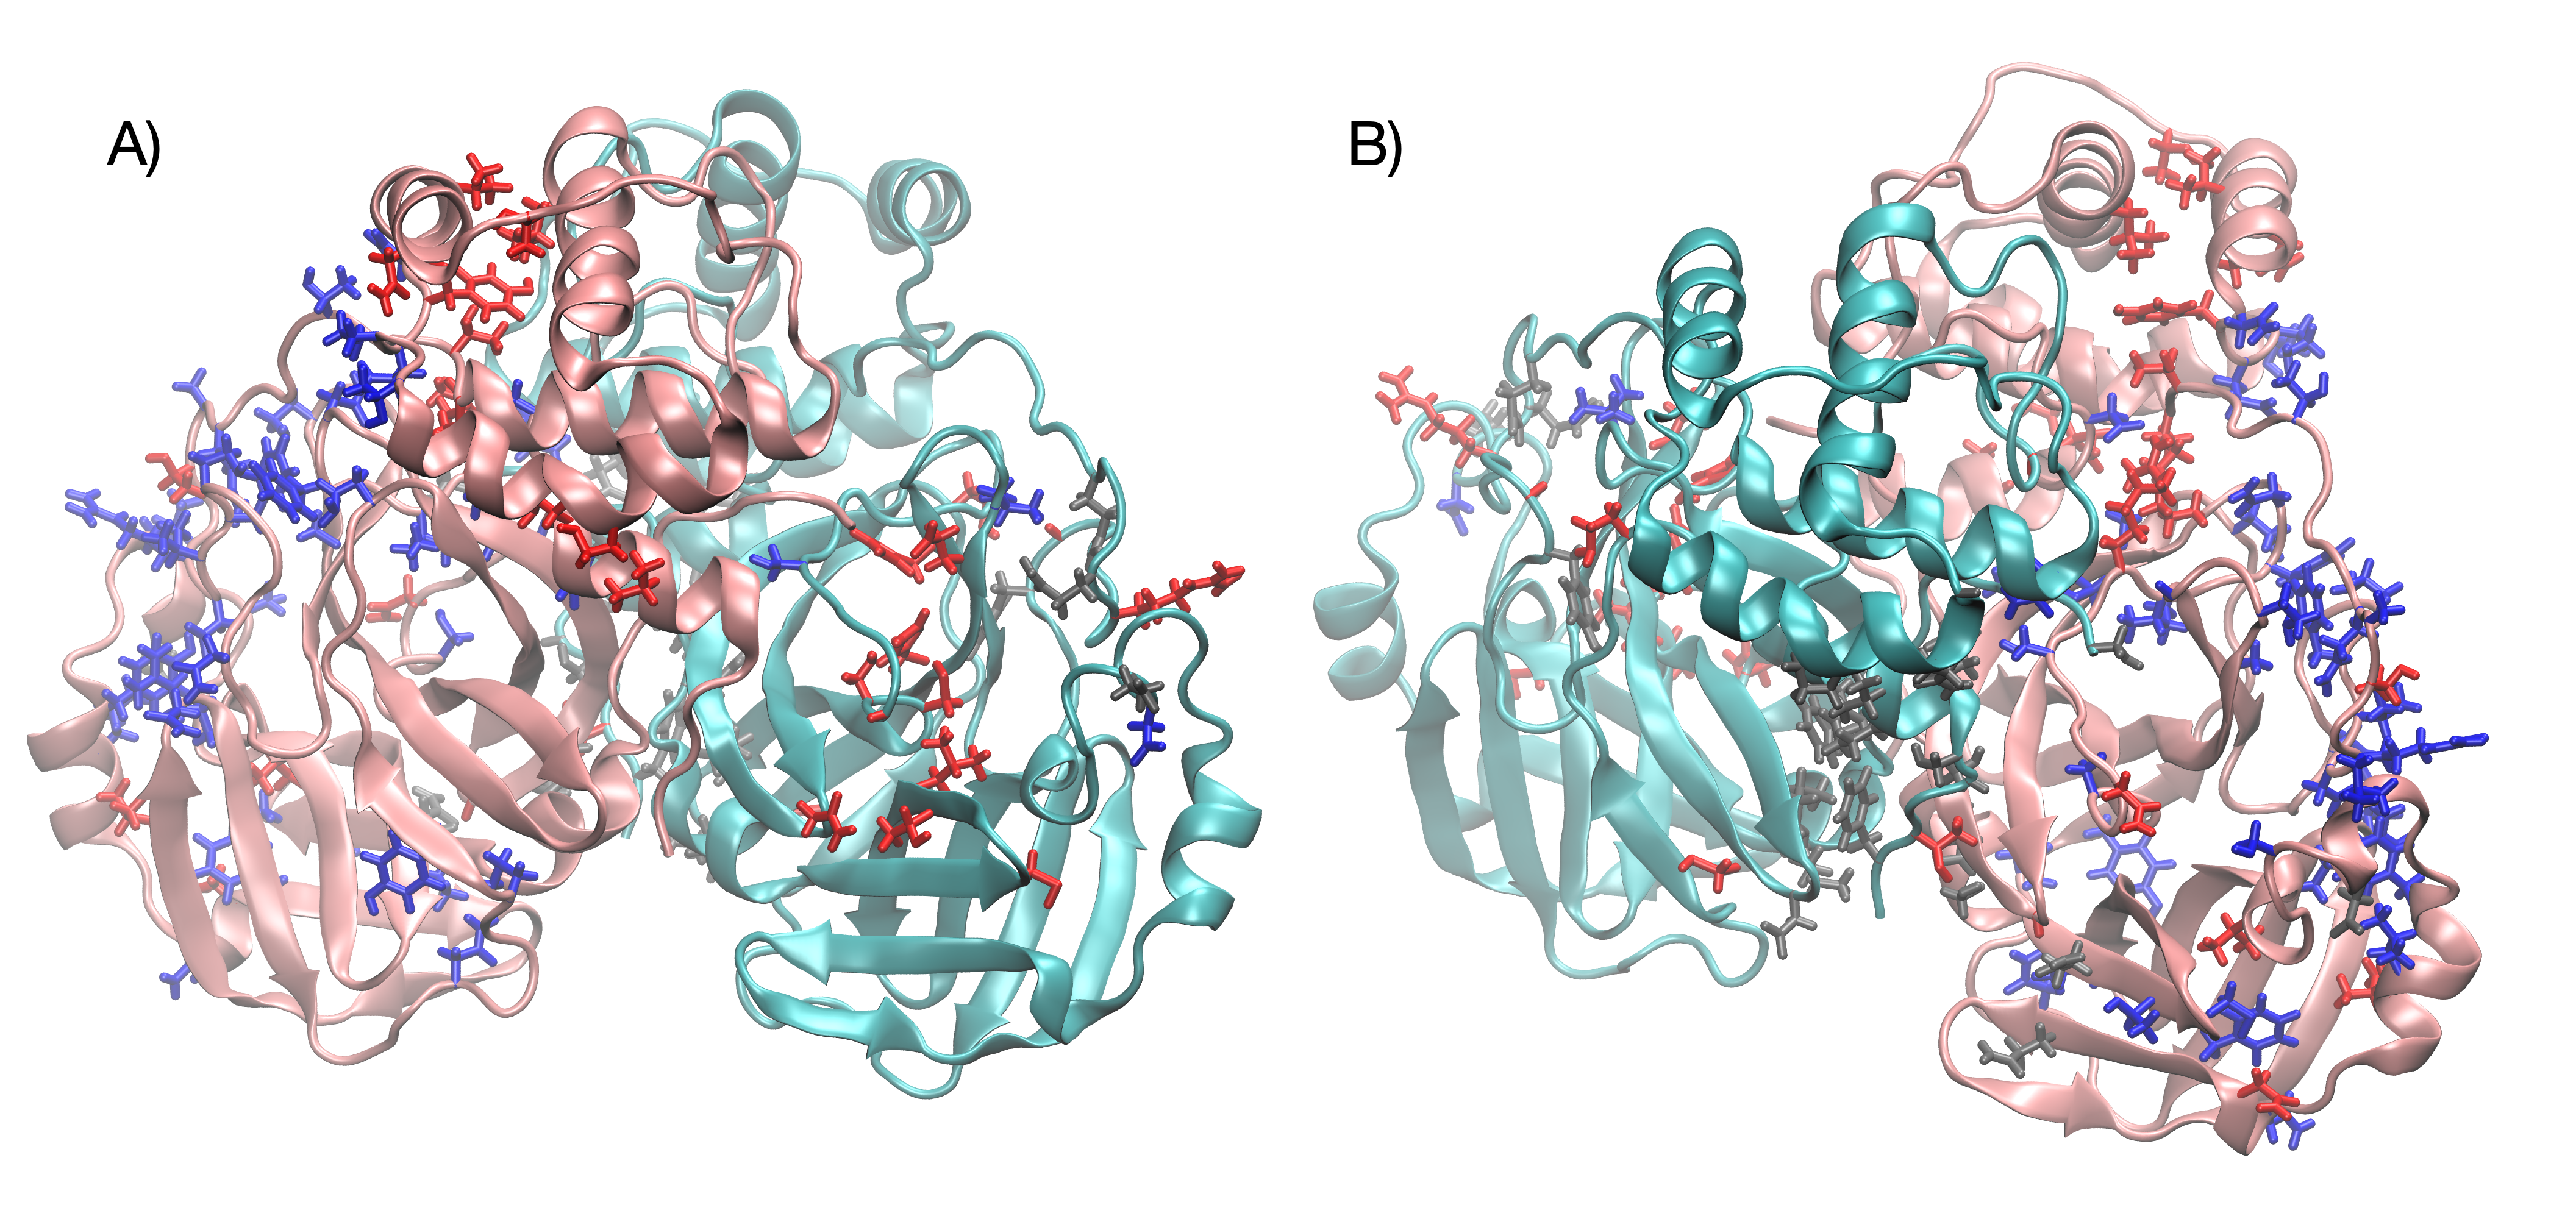
\includegraphics[width=0.6\linewidth]{images/fig_6_exposon_combined.png}
\caption{The three largest exposons are colored in blue, grey, and red. Chain A is shown in cyan and chain B in pink. shown in A, and flipped 180 degrees in B}
\label{fig:view}
\end{figure}

\subsection*{Discovery of slow motions}

In order to find a good set of internal coordinates or features to discover rare event motions in the $M_{pro}$ a filtered set of distances was created. Distances can be good at capturing interactions between non-sequential residues and especially between domains. Distances between monomers were not considered and the two monomers were treated as two separate trajectories of the same protein. This has been done before on other large viral systems, using the multiple copies of a protein in a system to obtain better sampling.\cite{perilla2017physical, hadden2018all} Residue pairs which never came close to being in contact (minimum distance > 10 Å) were filtered out, as well as residue pairs whose distance never changed ( standard deviation of < 0.35 Å). A visualization of these distances is shown in supplemental figure 1. Loosening these cutoffs to include almost double the amount of distances lowered the vamp-2 score, indicating that these additional distances added only noise and no signal to the calculation. Using pairwise distances between every fifth residue, backbone dihedral angles, or solvent accessible surface area per residue all have lower vamp-2 scores indicating that they don't capture the rare event motions well. Including sidechain torsions in addition to backbone torsions raises the vamp-2 score, which many indicate that there are some rare event sidechain motions slower than the backbone motions.

Tica performed on the filtered distances shows several motions which occur only once. These motions are also asymmetric, they occur in only one monomer. Independent component 1 (IC 1) and IC 2 both occur only in monomer B at 90 $\mu$S (figure 1). Independent component 1 is the folding of a helix in the linker region between domains II and III (residues 188 to 194). The loop flips out away from the protein, folds, then comes back in (figure 2). This loop folding is accompanied by residues 138, 139, and 140 moving closer to the strand-loop-strand residue 116 to 123. IC 1 and 2 happen concurrently and IC 2 has has is best captured by a motion of residue 144 away from residue 172 and toward residue 41. The linker loop is in close proximity to the active site sitting right at the interface between domains I and II. There is crystal structure evidence of this conformation. The related coronavirus, infectious bronchitis virus (IBV), which causes avian coronavirus was crystallized with three subunits in the asymmetric unit; a symmetric dimer, and a third monomer bound to the side of the dimer. This third monomer (chain C of pdbid: 2Q6D) also has this linker helix. It also has domain III shifted away from domain I and II.

Independent component 3 is residue 143 moving toward residue 167 to 172 and getting further from residues 19 and 20. Pro122 and Leu144 get closer, and Gly143 and Glu166 get closer. IC3 happens only once and only in chain A at about 29 $\mu$S into the simulation.

Since phi, psi, chi-1, and chi-2 dihedral space has a very high vamp-2 score, it was also examined. The top independent component from tica in phi, psi, chi-1, and chi-2 dihedral angle space captures the same motion that occurs in monomer B at 90 $\mu$S. This IC 1 correlates best to chi-1 of Phe291 in domain III. The next strongest correlations are in His172, Gly138, Glu166, His172, and Ser144 all very close together in domain 2. IC2 is also a monomer B at 90 $\mu$S and has correlations to Phe291, Tyr239, and Val233 in domain III, as well as Tyr101, Asp187, Tyr126, Phe140, Phe159, Leu141, and Glu166. This suggests domain II and III are moving together. The linker helix (residues 188 to 194) formation is IC 3. 

Another rare event of interest is the movement of the C-terminus (residue 306) to make contact with the catalytic residues. This occurs once for each protomer in the simulation. This conformation is necessary for self cleavage.\cite{muramatsu2016sars, noske2020crystallographic}

Making a full Markov state model of the $M_{pro}$ dynamics with good statistics was not possible due to the slowest motions only occurring once. This has also been reported by others. \cite{carli2020candidate, cocina2020sapphire}

\subsection*{Correlated motions}

Correlated motions were discovered using a mutual information analysis. First, correlated motions were examined using both chain A and chain B as two different trajectories of the same protein. The strongest correlations are seen near the active site. Residues 40 to 53, which includes the catalytic His41, have strong correlations with itself (40 to 53), 136 to 146, 166 to 172, and 185 to 192. The correlations around 136 to 146 are strongest around residue 41 and 42. The second area with strong correlations is 136 to 146, which includes the catalytic Cys145. It has strong correlations with residues 2 to 5, residue 27, 40 to 51, with itself (128 to 146), with 163 to 173, 185 to 193, 196 to 197, 232 to 233, 239 to 240, and 299 to 304. There are some additional correlated motions outside the regions of the catalytic residues but these residues all have additional correlated motions with the catalytic residues. Residues 163 to 173 have correlated motions with itself, as well as with 183 to 193. Similarly 185 to 193 has correlated motions with itself and 168 to 173.

Residues 163 to 173 is the strand loop strand motif involving $\MakeUppercase{\beta}$-strands 12 and 13. Notably it includes His166 which has been indicated in substrate binding. Residues 185 to 193 starts at the loop at the end of domain II and continues into the linker loop between domains II and III. This is the area where the linker loop forms in chain B. Residues 196 and 197 are at the very end of the linker loop right before domain 3. Residues 232 to 233 are in Helix 8 or domain III. This helix is quite far from the active site but yet still has very strong correlations with Cys145. Residues 239 to 240 are right after helix 8. During the simulation These residues start to form a parallel $\MakeUppercase{\beta}$-strand interaction with residues 198-200 in chain A.

Next, Correlated motion were examined on the full dimer (figure 4B). These motions were not the same for monomer A and B and did include correlations between monomers. The active site of chain A has slightly stronger correlations but these are constrained to a smaller number of residues. Chain B has a larger number of residues involved in correlated motions. This may be due to larger conformational change away from the starting structure in chain B. The 163 to 173 and 185 to 193 had much stronger correlations with the catalytic residues within chain B then they did in chain A. Residues 40 to 53 of chain A sees correlations to the C-termini of chain A, and weak correlations to 40 to 53, 136 to 146, 166 to 172, and 185 to 192 of chain B. Residues 136 to 146 of chain A have strong correlations with the C-terminus of A, the N-terminus of B, 232 to 233 of chain B, 239 to 240 of chain B, and the C-terminus of B. There are also weak correlations to 40 to 53 and 136 to 146 of chain B.

Chain B has more correlations within chain B, but chain B's catalytic residues only have weak correlations with the catalytic residue regions of chain A.

Exposons were calculated and the largest three are shown (figure 6). The exposons are shown from largest to smallest in blue, red, and grey respectively. The largest exposon (shown in blue) is the large set of residues which have their solvent exposure change when the linker helix folds. The next largest pocket (shown in red) primarily involves the active site of chain A, but also involves many residues in domain III. There is a channel formed in domain 3 with Lys137, Arg131, Ile200, Thr199, Thr239, Leu272, Ala234, Val233, and Thr225. The active site of chain A interacts with the C-termini of chain B which touches the channel at the interface of domain II and III. The third larges exposon (shown in grey) is an opening between the two protomers ant the domain II, domain II interface. The fourth largest exposon (data not shown) is the active site of chain B. 

\subsection*{Single monomer activation}

The literature has evidence that Sars-cov\cite{chen2006only} and Sars-Cov-2 has only one $M_{pro}$ monomer active at a time. The asymmetric motions seen here and seen in other $M_{pro}$ simulations\cite{inizan2021high} could be a conformational change away from a symmetric dimer imposed by crystal symmetry to a structure where one monomer is active-like and one is inactive like. The crystal structure (pdbid: 1UJ1) was seen with a $3_{10}$ helix in residues Ser139, Phe140, Leu141 in only one protomer which is believed to be a signal of inactivation. Here in Chain B Phe140 goes through a large conformational change early in the simulation (figure 7). Phe140 however does not fully flip out toward the other monomer to form a $3_{10}$ helix. Instead it moves closer to Glu166 on the same protomer.

The distance between 166 and 172 increases in the last 10 $\mu$S of chain B. This breaks the $\MakeUppercase{\beta}$-strand interaction between strand 12 and 13. The oxyanain loop (residues 139 - 145) goes through a large conformational change. This has also been seen in a $M_{pro}$ crystal structure. \cite{fornasier2021novel} The change seen here is not quite the same as the two largest halmarks, two consecutive b-turns with hydrogen bonds between Ser139-CO and Gln142-NH and between Leu141-CO and Ser144-NH, were not stable in this simulation

\section*{Discussion}

The $M_{pro}$ of Sars-CoV-2 is an extremely promising drug target with several open questions. The simulation here shows many changes near the active site. The folding of the linker helix creates less space in the S4 and S5 pockets. Substrate would be less likely to bind to this conformation. Neutron diffraction revealed that Cys44 side chain is likely to be deprotonated (S-) where here it is protonated (S+)\cite{kneller2020unusual}. In chain A Cys44 stayes burried but in chain B Cys44 pushes away from its hydrophobic pocket breaking the helix from 43 to 46 this may be responcible for the change in conformation of 46 to 53 which also changes the contacts with the linker loop. The IBV linker loop did not come with a conformational change in residues 43 to 53. Alignment of many $M_{pro}$ crystal structures shows heterogeneity in the residues 43 to 53 region. \cite{jaskolski2021crystallographic} Alignment of structures crystallized at different temperatures also shows large differences in this region

The C-termani flips away from the other protomer. The C-terminus is unresolved in many $M_{pro}$ crystal structures and is flexible in many others.\cite{jaskolski2021crystallographic} Two structures have been seen with this comformation 6xhmA and 7jkvB
(dig into what is IC3 more)

Correlated motions show the active site is the most dynamic part of this protein, which is not surprising, the active site needs correlated motions to cleave substrate. The motions of the active site appears to be connected to motions of many other regions of the protein. The residue 166 to 172 region of Domain II is adjacent to the active site and has been implicated in single monomer activation. The instibility in this region could also be caused by the improper protonation of residues His163 and His164, though the chain A monomer remains stable.

The residue 136 to 146 region has correlated motions with both termini (residues 2 to 5 and residues 299 to 304) the same protomer as well as on the other protomer. This could allow for motions to be transfered to the other protomer. It is also possible that this large group of residues moving as a unit is needed for cleavage motions which could explain why both protomers cannot cleave substrate at the same time. A substrate bound protomer could inhibit motions needed for the other protomer to bind a second substrate or to cleave substrate.

Residues 232 to 233 having correlated motions with Cys145 suggests that domain III can impact motions in the active site. It's not fully clear how motions this far away could have an impact on each other. However the inhibitors x0390 and x0464 bind at the interface of domain II and III quite close to residues 232 to 233 and inhibit activity without affecting dimerization. \cite{el2020allosteric} This would imply that changes to domain III can affect motions in the active site.

compare to other simulations

The correlated motions presented in figure 5 don't have great agreement with the correlated motions presented in \cite{sztain2020elucidation}. \cite{sztain2020elucidation} looks for correlated motions in Cartesian coordinate space. This has the disadvantage of needing a good alignment of frames and having a good global and local alignment at the same time is very difficult. Correlations in Cartesian coordinate space show subdomains of the protein which move together. Using dihedral space eliminates any noise from rotational and translational movement and can better capture larger non-linear conformational changes.

\LaTeX{} formats citations and references automatically using the bibliography records in your .bib file, which you can edit via the project menu. Use the \verb|\cite| command to insert a citation, like this: \cite{Chen_Nicholson00} Multiple citations can be given as \cite{Stiles_Bartol01,el-Kareh_etal93,Callaghan91}. You can use either BibTeX or biblatex: see the following subsections.

If your manuscript is accepted, the Biophysical production team will re-format the references for publication. \emph{It is not necessary to format the reference list yourself to mirror the final published form.}

\subsection*{Using bibtex} 
This is the default. Specify your \texttt{.bib} file with \verb|\bibliography{sample}| (the extension is unnecessary) near the end of your manuscript, where you want the references list to appear.

\subsection*{Using biblatex} 
Pass the \texttt{biblatex} option to the \verb|\documentclass| declaration, then specify your \texttt{.bib} file name in the \emph{preamble}: \verb|\addbibresources{sample.bib}| (the extension is necessary). Write \verb|\printbibliography| near the end of your manuscript where you want the references to appear.

\section*{Conclusion}

Sed ut perspiciatis unde omnis iste natus error sit voluptatem accusantium doloremque laudantium, totam rem aperiam, eaque ipsa quae ab illo inventore veritatis et quasi architecto beatae vitae dicta sunt explicabo. 

\section*{Author Contributions}

Author1 designed the research. Author2 carried out all simulations, analyzed the data. Author1 and Author2 wrote the article. 

\section*{Acknowledgments}

We thank G. Harrison, B. Harper, and J. Doe for their help.

% Uncomment if using bibtex (default)
\bibliography{sample}

% Uncomment if using biblatex
% \printbibliography

\section*{Supplementary Material}

An online supplement to this article can be found by visiting BJ Online at \url{http://www.biophysj.org}.

\begin{figure}[hbt!]
\centering
% image made using starting structure: https://github.com/jgpattis/Desres-sars-cov-2-apo-mpro/blob/master/DESRES_protease_chainid.pdb
% and tcl file from: https://github.com/jgpattis/Desres-sars-cov-2-apo-mpro/blob/master/filter_distance_01.py
%\graphicspath{ {./supplemental_figures/} }
% fdis-visualization.png
% overleaf does not like this image for some reason
\includegraphics[width=0.6\linewidth]{supplemental_figures/fdis-visualization_smaller.png}
\caption{A visualization of the 2389 distances included in the filtered distances featurization}
\label{fig:view}
\end{figure}

\begin{figure}[hbt!]
%feature-selection
% figure created with: https://github.com/jgpattis/Desres-sars-cov-2-apo-mpro/blob/master/plot_vamp_score_04.py
\centering
\includegraphics[width=0.6\linewidth]{supplemental_figures/sup_fig_2_vamp_score.png}
\caption{The Vamp-2 score of different feature options scored on the top 10 eigenvalues of the VAMP dimentionality reduction while running 20 iterations of 50:50 shuffle split cross validation}
\label{fig:view}
\end{figure}

\begin{figure}  %[hbt!]
\centering
% green48_iceblue19.png
\includegraphics[width=0.6\linewidth]{supplemental_figures/green48_iceblue19_smaller.png}
\caption{Alignment of chain B of cluster 48 (green) and cluster 19 (iceblue)}
\label{fig:view}
\end{figure}

\begin{figure}[hbt!]
% mutual-information-average
% raw images: raw_images/dmi_bothchain_35_15_view1_snap.png
% raw_images/dmi_bothchain_35_15_view2_snap.png
% averaged_MI_image.graffle
\centering
\includegraphics[width=0.6\linewidth]{supplemental_figures/Averaged_MI_image_smaller.png}
\caption{visualization of residue pairs with high correlation (red lines) MI over 0.35 and moderate correlation (blue) MI over 0.15 averaged between the two chains A) AND B) rotated 180 degrees}
\label{fig:view}
\end{figure}

\begin{figure}[hbt!]
%mutual-information-dimer
% raw images: raw_images/mut_info_35_15_front_good.png
% raw_images/mut_info_35_15_back.png
% raw_images/dimer_MI_image.graffle
\centering
\includegraphics[width=0.6\linewidth]{supplemental_figures/dimer_MI_image.png}
\caption{visualization of residue pairs with high correlation (red lines) MI over 0.35 and moderate correlation (blue) MI over 0.15 for the dimer A) AND B) rotated 180 degrees}
\label{fig:view}
\end{figure}

\end{document}
